\documentclass[11pt,a4paper,fleqn]{article} 
%%%%% general %%%%%
\usepackage[T1]{fontenc} 
\usepackage{geometry}
\geometry{a4paper, top=20mm, left=20mm, right=20mm, bottom=20mm,headsep=10mm, footskip=12mm}
\usepackage[singlespacing]{setspace} %Zeilenabstand
\usepackage{xspace} %Befehle fuer Bezeichner, damit danach Leerzeichen
%%%%% lists %%%%%%

\usepackage[alwaysadjust,flushleft]{paralist}
\usepackage{enumerate}
%%%%% graphics and tables %%%%%
%\usepackage{graphicx}
\usepackage{subfigure}
\usepackage{booktabs}
\usepackage{multirow}

%\usepackage{longtable}
\usepackage{rotating}
%\usepackage{placeins}
\usepackage{flafter} %no floating object appears in the text above the position where it is defined
%\usepackage[font=small,labelfont=bf]{caption} 
\newcommand{\ra}[1]{\renewcommand{\arraystretch}{#1}}
\usepackage{tikz}
\usepackage{pgfplots}

%%%%% Mark changes %%%%%
%\usepackage{soul}
%\setstcolor{red}
%\usepackage{cancel}
\usepackage[final]{changes}

%%%%% bibliography %%%%%
\usepackage{natbib}
\bibliographystyle{abbrvnat}
\bibpunct[, ]{(}{)}{,}{a}{}{,}%
\def\bibfont{\small}%
\def\bibsep{\smallskipamount}%
\def\bibhang{24pt}%
\def\newblock{\ }%
\def\BIBand{and}%
%%%%% math and algorithms %%%%%
\usepackage{amsmath}
\usepackage{amssymb}
%\usepackage{algorithm}
\usepackage{array}
%\newcolumntype{H}{>{\setbox0=\hbox\bgroup}c<{\egroup}@{}}
\usepackage{algorithmic}
\usepackage{fixltx2e} % text super and subscripts
%%%%% color %%%%%%
\PassOptionsToPackage{usenames,dvipsnames}{color}
%\usepackage[usenames,dvipsnames]{color}
%%%%% hyperref %%%%%%
%\usepackage{url}
%\usepackage{preview}
%\usepackage{breakurl} \% break long urls
%\usepackage[colorlinks,linkcolor=Goldenrod,citecolor=Brown]{hyperref}
\usepackage{hyperref}
% \hypersetup{
%     bookmarks=true,
%     unicode=false,
%     pdftoolbar=true,
%     pdfmenubar=true,
%     pdffitwindow=false,
%     pdfstartview={FitH},
%     pdftitle={My title},
%     pdfauthor={Author},
%     pdfsubject={Subject},
%     pdfcreator={Creator},
%     pdfproducer={Producer},
%     pdfkeywords={keyword1} {key2} {key3},
%     pdfnewwindow=true,
%     colorlinks=true,
%     linkcolor=black,
%     citecolor=black,
%     filecolor=black,
%     urlcolor=black
% }


\pgfplotsset{compat=1.12}
\allowdisplaybreaks[4]
%%%%% Math Operators %%%%%
\DeclareMathOperator*{\argmin}{arg\,min}
\DeclareMathOperator*{\argmax}{arg\,max}

\usepackage{atbegshi}% http://ctan.org/pkg/atbegshi
\AtBeginDocument{\AtBeginShipoutNext{\AtBeginShipoutDiscard}}


\begin{document}

\onehalfspacing
\title{Optimizing Air Cargo Handling at an International Airline Hub for AbOvo \\ MSc Data Analytics and Decision Science RWTH Aachen University} 
\author{Ilkim Canoler \\ Luckshan Sivakumar \\  Nikhil Kulkarni \\ Karthikeyan Ramasubbu \\ Shekhar Dure}
$\newline$
$\newline$
\date{12th June 2019}
\maketitle
\thispagestyle{empty}


$\newline$
\begin{abstract}
	In this study, an operational planning problem in the air cargo industry is being tried to be solved. For all shipments in an international airline hub that need to catch their related flight on time, a mathematical model was constructed.  Working with our industrial partner AbOvo, we formalize the problem constraints and our objective. Besides, the necessary data is collected from AbOvo and we started working on it simultaneously. We are trying to establish a comprehensive view of tasks in an air cargo terminal and develop a suitable solution apporoach. Furthermore, our goal is to solve this model by using Gurobi solver as a full planning puzzle. In this paper, all explanations and details about our mathematical model and the data we have, can be found.
	
\end{abstract}

\clearpage
\pagenumbering{arabic} 

\newpage

\tableofcontents

\newpage

\section{Introduction}
\label{sec:introduction}

$\newline$
An international airline hub needs to plan the air cargo movement so that all shipments catch their connecting flights or road connections. Air cargo shipments are transported in so-called unit load devices (ULDs). A ULD contains many shipments which need to go different final destinations. Hence, at the first step of the whole process, the incoming ULDs are broken down at the arrival. Here in the breakdown zone (BD), ULDs have to be unpacked and seperated. The seperate shipments are transported in the warehouse to wait for the build up call. These shipments are then moved to packing area which is called buildup zone (BU). At the end, outbound ULDs are constructed with these shipments and they are taken to the outbound flight for loading. All zones have different attributes such as number of workstations, capacities, transportation times between zones and the warehouse. Shipments also have different attributes such as priority and weight. Regarding all the attributes, constraints and the parameters which are stated in detail in problem description, the goal of the optimization process is to build up all ULDs as soon as possible to make them catching their connections.
$\newline$


%\noindent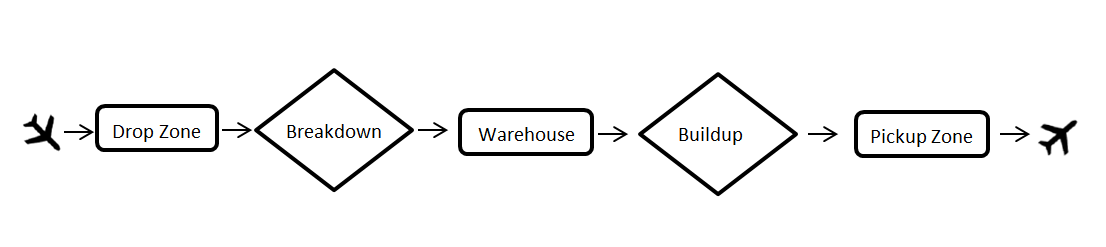
\includegraphics[width=18cm]{1_process.png}\qquad
$\newline$

\begin{figure}[hbt!]
	\centering
	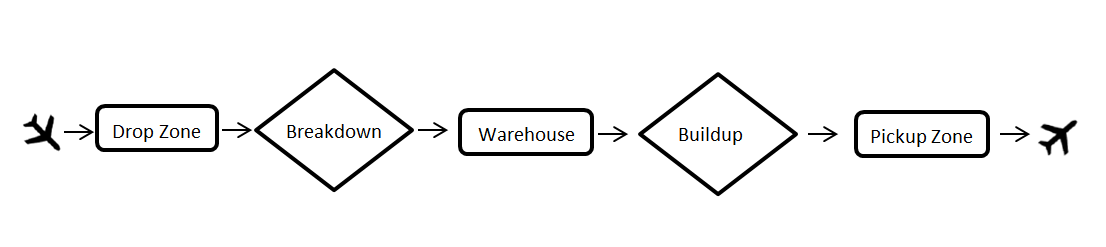
\includegraphics[width=170mm,scale=1.5]{1_process.png}
	\caption{The Process That Takes Place at a Hub}
	\label{fig:The Process That Takes Place at a Hub}
\end{figure}

$\newline$

\newpage

\section{Problem Description}
\label{sec:problemdescription}

$\newline$
The process of one shipment begins in drop zone when it comes to the airport in an inbound ULD. ULDs are unloaded from an aircraft by the ground handling agent and placed in a drop zone (not part of our planning puzzle). There are 4 drop zones and each drop zone has different number of workstations. Each ULD has a scheduled arrival and at a later stage an actual arrival time. From drop zone, each ULD has to be taken to the breakdown zone to get unpacked. Our problem also starts here. There are different distances between each drop zone and each breakdown zone. The sample distances between some of the drop zones and some of the BD zones are given below in the table:

$\newline$
%\noindent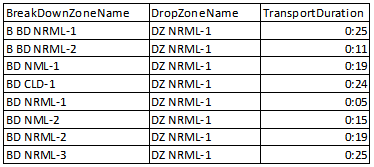
\includegraphics[width=12cm]{distances_drop_bdzone.png}\qquad

\begin{figure}[hbt!]
	\centering
	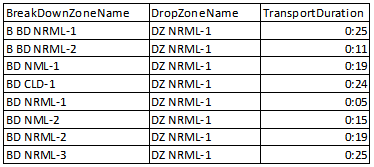
\includegraphics[width=100mm,scale=1.5]{distances_drop_bdzone.png}
	\caption{Sample Distances Between Drop Zone and Break Down Zone}
	\label{fig:Sample Distances Between Drop Zone and Break Down Zone}
\end{figure}

$\newline$
In BD zone, ULDs are seperated into shipments. There are 12 different BD zones in the hub. So they are located at different places of the airport. Thus all BD zones have different attributes. Attributes related to BD zones are below: 

\begin{itemize}
	\item Different characteristics for each BD zone for example some of the BD zones are for animals, some of them are for cooled products and the others are normal BD zones.
	\item Different number of workstations within the BD zone.
	\item Different transportation times to the warehouse.
	\item Different handling times per ULD.
\end{itemize}

\begin{figure}[hbt!]
	\centering
	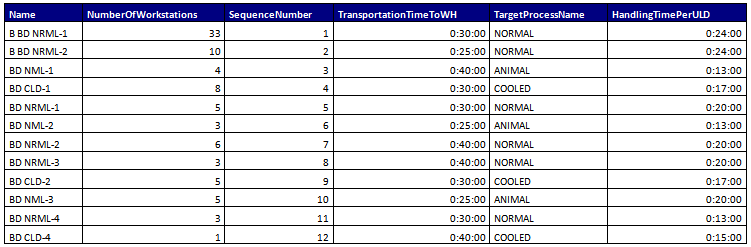
\includegraphics[width=150mm,scale=1.0]{BDZones.png}
	\caption{Break Down Zone Attributes}
	\label{fig:Break Down Zone Attributes}
\end{figure}

%\noindent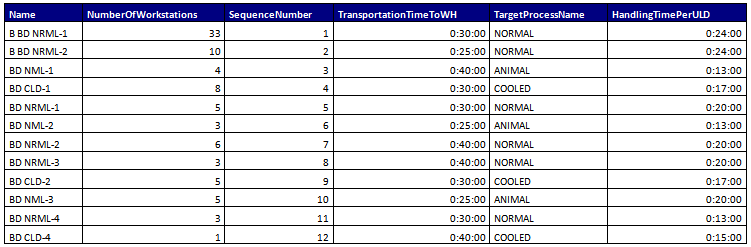
\includegraphics[width=30cm]{BDZones.png}\qquad

$\newline$
Within the BD zone, the decision needs to be taken in which order the ULDs should be unpacked. ULDs need to be broken down early enough, so all shipments can make their connections or promised pickup time. There are 3 different shipments within the hub. Cooling products, normal products (NRML) and animals (NML). Also each shipment has different priorities in these BD zones. Because some of the shipments may be animals or cooled products which are mentioned above and need to be processed before the regular shipments. ULDs contain a shipment with a high priority, need to be unpacked earlier than the others. Each shipment within the ULD is either in transit and needs to catch the connecting flight or will be further transported on the road usually by truck (not part of our planning puzzle) or is picked up from the warehouse by a customer. When the shipments are in transit and unpacked, depending on the scheduled departure time of the connection flight on which cargo is booked, it is either stored temporarily in the warehouse or directly sent to build up process. The warehouse (WH) is fully automated and with the assumption, that there are never capacity constraints in the WH. As soon as enough stock is available in the storage WH to build up one ULD for a specific aircraft, these can be requested to be provided to the BU zone.

$\newline$
In a next step the shipments are built up again to ULDs depending on their connecting flight. This is done within a build up zone (BU zone). A departing aircraft type has a link to a specific BU zone, so with the provided information which aircraft the shipment should go on, the BU zone is known. Here again a shipment with a high priority has to be built up earlier then the other shipments. There are 8 different BU zones and each BU zone has different number of workstations within. At each work station one ULD can be built up at the same time. The shipments are provided from the storage WH to the chosen work station. If the building up of two ULDs for the same aircraft are planned at one work station, it is not allowed to build up a ULD for a different aircraft in between, even if there is some idle time. The reason is that after building up one ULD there might be some shipments with the same destination left. It should be avoided to move those around, so they would stay at the work station for the build up of the next ULD for the same aircraft. From each BU zone, there are different transportation times to each flight. In addition to this, there are different default processing times for each flight which is also given in the data. This means each ULD has additional processing time before the regarding flight. Here for all ULDs, the capacity is the same which is 400 kg. For some of the flights, there is a pre-processing buffer time necessary to consider. Sample tables related to these characteristics are given below for a clear understanding:

\begin{itemize}
	\item Different handling times and transport times from the WH for each BU zone.
	
	\begin{figure}[hbt!]
		\centering
		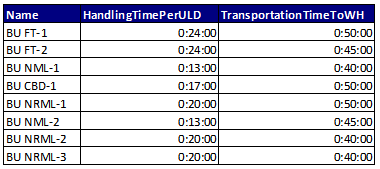
\includegraphics[width=100mm,scale=1.5]{buzone_data1.png}
		\caption{Handling Times and Transportation Times from Warehouse to BU Zones}
		\label{fig:Handling Times and Transportation Times from Warehouse to BU Zones}
	\end{figure}

\end{itemize}

	%%\noindent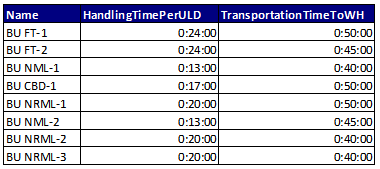
\includegraphics[width=14cm]{buzone_data1.png}\qquad

\begin{itemize}

	\item Sample workstations within some BU zones.
	
	\begin{figure}[hbt!]
		\centering
		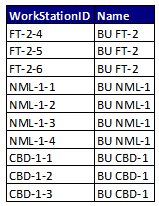
\includegraphics[width=40mm,scale=1.0]{sample_ws_bu.png}
		\caption{Workstations in BU Zones}
		\label{fig:Workstations in BU Zones}
	\end{figure}
	%%\noindent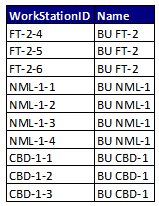
\includegraphics[width=8cm]{sample_ws_bu.png}\qquad

\end{itemize}

\newpage

\begin{itemize}

	\item Sample flights related to some BU zones and the transportation time between the flight and the BU zone.
	
	\begin{figure}[hbt!]
		\centering
		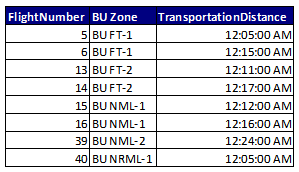
\includegraphics[width=90mm,scale=1.5]{sample_bu_flight.png}
		\caption{Sample Flights Related to BU Zones and Transpotation Times}
		\label{fig:Sample Flights Related to BU Zones and Transpotation Times}
	\end{figure}
	%%\noindent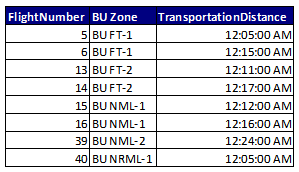
\includegraphics[width=10cm]{sample_bu_flight.png}\qquad

\end{itemize}

\begin{itemize}

	\item Pre-processing buffer times for the flights.
	
	\begin{figure}[hbt!]
		\centering
		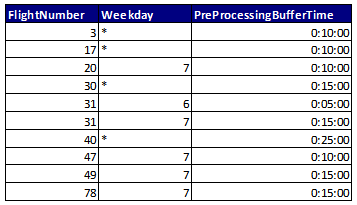
\includegraphics[width=90mm,scale=1.5]{preprocess_time.png}
		\caption{Pre-Processing Times of the Flights}
		\label{fig:Pre-Processing Times of the Flights}
	\end{figure}
	%%\noindent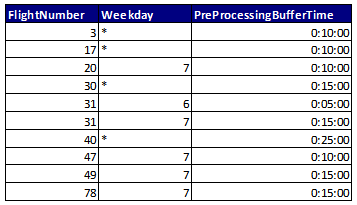
\includegraphics[width=10cm]{preprocess_time.png}\qquad
	
\end{itemize}

The goal is to build up all ULDs as soon as possible to make the connections, while the work should be processed in batches, to avoid unnecessary transportation within the BU zone.

\newpage


\section{Mathematical Model for the Problem}
\label{sec:mathmodel}

Our mathematical model for this problem is a combination of two parts of the puzzle which are Break Down Zone and the Build Up Zone. According to this, the model has different parameters, decision variables, constraints and objective function components for different zones and we treated the problem first as seperate models. At the end, overall model can be seen with both puzzles included. 

$\newline$ 

\begin{figure}[hbt!]
	\centering
	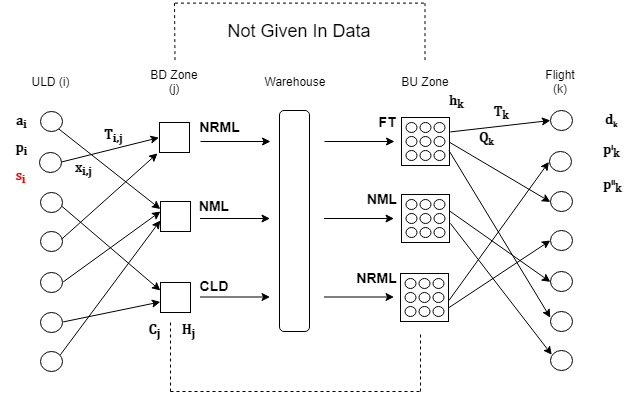
\includegraphics[width=150mm,scale=1.5]{Aircargo_overall.png}
\end{figure}


\subsection{Break Down Process}
\label{sec:ParamBDZone}

In BD zones, our model has arrival time parameters for each ULD. Similar to this, each BD zone has its own capacity, handling time and transportation time from drop zone. Each ULD is a part of the ULD set I and each BD zone is a part of the BD zones set J. Time is discretized into minutes in set T.

\begin{equation*} ${\color{black} ULD i}$ {}  \in {}  ${\color{black}I}$ {} = {} ${\color{black}\{1,2,3,...,N\}}$  \end{equation*} 
\begin{equation*} ${\color{black} BD zone j}$ {}  \in {}  ${\color{black}J}$ {} = {} ${\color{black}\{1,2,3,...,M\}}$ \end{equation*} 
\begin{equation*} ${\color{black} Time horizon t}$ {}  \in {}  ${\color{black}T}$ {} = {} ${\color{black}\{1,2,3,...,T\}}$ \end{equation*} 


${\color{black}a_{i}}$ : Arrival time of ULD ${\color{black}i}$ in drop zone 

%$\textcolor{black}{s_{i}}$ : Idle time spent by ULD ${\color{black}i}$ in drop zone

%$\textcolor{black}{p_{i}}$ : Priority of ULD ${\color{black}i}$

${\color{black}c_{j}}$ : Capacity of BD zone ${\color{black}j}$

$\textcolor{black}{h_{j}}$ : Handling time in BD zone ${\color{black}j}$

$\textcolor{black}{T_{ij}}$ : Time taken to transport an ULD ${\color{black}i}$ to BD zone ${\color{black}j}$

$\textcolor{black}{T_{j}}$ : Time taken to transport shipments from ${\color{black}i}$ to BD zone ${\color{black}j}$ to Warehouse

$\newline$

\subsubsection{Decision Variables for Break Down Process}
\label{sec:DVBDZone}

In the Break Down zone, the decision needs to be taken which ULDs should be assigned to which BD zone at which time. For this reason, the decision variable has to be binary. 1 for the ULD i is assigned to BD zone j at time t, 0 for the ULD i is not assigned to BD zone j at time t. 

$\newline$

$\textcolor{black}{x_{ij}^{t}\in\{0,1\}, \forall {i \in I, j \in J, t \in T}}$ : if a ULD i is assigned to BD zone j at time t or not.

$\newline$

\subsubsection{Constraints for Break Down Process}
\label{sec:constraintsBDZone}

For BD processes we have several constraints. The first one (1) is the assignment constraint which means all ULDs have to be assigned to exactly one BD zone  and the second one (2) is the capacity constraint. 


%\begin{align}
%\sum_{i \in {I}} x_{ij}^{t} \le c_{j} \qquad \forall j \in J, \forall t \in T 
%\end{align}
%\begin{align}
%\sum_{j \in {J}} x_{ij}^{t} = 1 \qquad \forall i \in I, \forall t \in T
%\end{align}

$\newline$

\begin{align}
\sum_{j \in J}\sum_{t=1}^{T-h_{j}+1} x_{ij}^{t} = 1 \qquad \forall i \in I
\end{align}

$\newline$
In the second constraint (2), we say that if ULD's in subset i are started to be processed at time t, no more ULDs than the remaining capacity of the BD zone j can start before $t + h_{j}$ , because the process of breaking down the current ULDs needs to be completed.
If ULDs in subset i start at t in BD zone j, then other ULDs are in $u \in I \setminus \{i\}$. In the first part of the constraint, we are calculating the remaining capacity for the BD zone at time t . For the second part of the constraint, we are stating that whatever will be assigned in next time period $t + h_{j}$ should be less than or equal to remaining capacity.

\begin{align}
c_{j} - \sum_{i \in I} x_{ij}^{t} \ge \sum_{u \in I \setminus \{i\}}\sum_{\tau = t}^{t+h_{j}-1} x_{ij}^{\tau} \qquad \forall t \in T, \forall j \in J
\end{align}

$\newline$

The effect is no more ULDs than the capacity of BD zone are assigned at any time.
We get starting time of ULD i : 
$\newline$
$t_{i,start} = \sum_{t=0}^{T-h_{j}+1} t . x_{ij}^t $

$\newline$
ULD i is broken down at time :

$\newline$
 $t_{i,end} =   \sum_{t=0}^{T-h_{j}+1}{\color{black}{(t + \sum_{j \in J}h_{j})}}$

$\newline$
At this phase, priorities are not considered in our model in BD zones.

$\newline$

\subsection{Build Up Process}
\label{sec:ParamBUZone}

During BU process, our model has several parameters for both of the flights and the time horizons. 

\begin{equation*} ${\color{black} Flight k}$ {}  \in {}  ${\color{black}K}$ {} = {} ${\color{black}\{1,2,3,...,K\}}$  \end{equation*} 
\begin{equation*} ${\color{black} Time horizon t}$ {}  \in {}  ${\color{black}T}$ {} = {} ${\color{black}\{1,2,3,...,T\}}$ \end{equation*} 

$\newline$

The first constraint is about available weight for a given time t and for a flight k which means the summation of the weights of the seperate shipments which are raedy to build up and waiting in the warehouse.

$\newline$

$avail_{kt}$ $\in$ $\mathbb{R}$

$\newline$

The second one is the due time of the build up process for a flight k.

$\newline$

$due_{k}$ $\in$ $\mathbb{R}$

$\newline$

The third one is the total shipment weight as a demand for a flight k.

$\newline$

$dem_{k}$ $\in$ $T$

$\newline$

The fourth one is the maximum number of ULDs building up simultaneously for a flight k. It actually means number of workstations which are working parallel. In practice we only want to build a limited number of ULDs for the same flight at the same time. This leaves more options and time to react to operational problems during build up and allows to build the ULDs on close-by workstations. Let maximum split denote the maximum desired number of parallel build-ups of a flight. Enforcing a hard limit in practice might lead to offloads for flights where the shipment arrives rather late such that the limit is too low to build all ULDs on time. In these cases we want to set a less restrictive limit.


As a suitable limit we choose the maximum required parallel build-ups, between any build-up period and the scheduled departure period of the flight, for which all shipments can be packed. For each period t, we determine the shipment weight arriving in the future (weight demand of flight k) $-$ (available weight at time t for flight k) and the weight that could be packed in the remaining time, if no parallel build-ups are allowed. Note that the number of ULDs that can be built sequentially in the time between t and due time for flight k, can be determined as (due date of flight k $-$ t $-$ 1) $/$ (duration to build a ULD for a flight k). The ratio of both gives us the required parallelism and its maximum over the periods the sought limit. If the required parallelism is less than the desired maximum split, we allow maximum split to be built in parallel.

$\newline$

$split_{k}$ $\in$ $\mathbb{N}$

$\newline$

The fifth parameter is the number of ULDs scheduled for a flight k. It means that total shipment weight for a flight k is divided into capacity which is 400 kg and gives us the valueof the parameter. 

$\newline$

$uld_{k}$ $\in$ $\mathbb{N}$

$\newline$

The sixth one is the duration in minutes for building a ULD for flight k. We actually know which BU zone is used for flight k before, that is why we do not consider here BU zone index.

$\newline$

$dur_{k}$ $\in$ $\mathbb{N}$

$\newline$

The seventh one is the weight of an ULD which is 400 kg as stated in the data.

$\newline$

$cap$ $\in$ $\mathbb{R}$

$\newline$

The last one is the number of workstations handling the ULDs during time t. It is for all flights in time horizon t.

$\newline$

$open_{t}$ $\in$ $\mathbb{N}$

$\newline$


\subsubsection{Decision Variables for Build Up Process}
\label{sec:DVBUZone}

The primary decision made by the model is the number of ULDs to start building at each
period. To calculate the objective value, we introduce further decision variables. One
part of the objective is to load as much as possible. There are two reasons that might
prevent us from achieving this goal: First, if not all ULDs can be scheduled for build-up.
Second, if a ULD is scheduled before enough shipment is available. We capture the effect of
each reason in one variable.

$\newline$

$\textcolor{black}{start_{kt}\in\mathbb{N}, \forall {k \in K, t \in T}}$ : Number of ULDs started to build at time t for a flight k $t \le due_{k} $ - $dur_{k}$

$\newline$

$\textcolor{black}{offload_{k}\in\mathbb{N}, \forall {k \in K}}$ : Number of NOT scheduled ULDs for flight k


$\newline$

$\textcolor{black}{dead_{kt}\in\mathbb{R} \ge 0, \forall {k \in K, t \in T}}$ : Lost weight of shipments on flight k if ULDs are built before enough shipments available at time t


$\newline$

\subsubsection{Constraints for Build Up Process}
\label{sec:constraintsBUZone}

There is no technical reason to restrict the number of ULDs that are
built in parallel for a segment. However, in practice there might occur problems during
a build-up when an item cannot be packed onto the planned ULD. In this case, the load
planner has to find another ULD with enough remaining capacity under massive time
pressure. The more ULDs that are not started yet, the more options and time he has
for replanning. Furthermore, if only a few ULDs for a segment are built in parallel, they
can be assigned to spatially close workstations. This might reduce transport distances
and improve overview during build-up. We note that, during a period t, the ULDs that
were started during period (t $-$ $dur_{k}$ $+$ 1) to period t are still work in progress. For each flight k we limit the number of simultaneously built ULDs by splitk as:

\begin{align}
\sum_{t' \in {T}} start_{kt'} \le split_{k} \qquad \forall k \in K, \forall t \in T
\end{align} $t - dur_{k} \le t' \le t$

$\newline$

The number of usable workstations is limited. As each workstation
can process one ULD at a time, we limit the number of simultaneously processed
ULDs during period t by $open_{t}$. To calculate this number for a point in time,
we sum up the ULDs of all flights that have been started during earlier periods and
are not finished yet:

\begin{align}
\sum_{k \in {K}}\sum_{t' \in {T}} start_{kt'} \le open_{t} \qquad \forall t \in T
\end{align} $t - dur_{k} \le t' \le t$

$\newline$

\subsubsection{Objective Function}
\label{sec:objBUZone}

While satisfying all the given constraints, we want to load as much cargo as possible. o maximize the load, we minimize the amount of weight the departing flight lost and the number of ULDs building up unassociated to the departing flight.

\begin{equation*}
\min \qquad {} (\sum_{k \in K} \sum_{t \in T} dead_{kt} + \sum_{k \in K} offload_{k})
\end{equation*}

$\newline$

%\subsection{Overall Model}
%\label{sec:overallModel}

%------------------------------------------------------------------------

%\begin{table}[h!]
%	\begin{center}
%		\caption{Drop Zone}
%		\label{tab:table1}
%		\begin{tabular}{l|c|c} % <-- Alignments: 1st column left, 2nd middle and 3rd right, with vertical lines in between
%			\textbf{Name} & \textbf{Workstations} & \textbf{Sequence}\\
%			\hline
%			& & \\
%			DZ NRML-1 & 6 & 1\\
%			DZ NRML-2 & 4 & 2\\
%			DZ NML-1 & 3 & 3\\
%			DZ CLD-1 & 5 & 4\\
%		\end{tabular}
%	\end{center}
%\end{table}

%\begin{table}[h!]
%	\begin{center}
%		\caption{Break Down Zone}
%		\label{tab:table1}
%		\begin{tabular}{l|c|c|c|c} % <-- Alignments: 1st column left, 2nd middle and 3rd right, with vertical lines in between
%			\textbf{Name} & \textbf{Workstations} & \textbf{Sequence} & \textbf{ToWH} & \textbf{HandTimePerULD}\\
%			\hline
%			& & & & \\
%			B BD NRML-1 & 33 & 1 & 0:30 & 0:24\\
%			B BD NRML-2 & 10 & 2 &  0:25 & 0:24\\
%			BD NML-1 & 4 & 3 &  0:40 & 0:13\\
%			BD CLD-1 & 8 & 4  &  0:30 & 0:17\\
%			BD NRML-1 & 5 & 5  &  0:30 & 0:20\\
%			BD NML-2 & 3 & 6  & 0:25 & 0:13\\
%			BD NRML-2 & 6 & 7  & 0:40 & 0:20\\
%			BD NRML-3 & 3 & 8  & 0:40 & 0:20\\
%			BD CLD-2 & 5 & 9  & 0:30 & 0:17\\
%			BD NML-3 & 5 & 10  & 0:25 & 0:20\\
%			BD NRML-4 & 3 & 11  & 0:30 & 0:13\\
%			BD CLD-4 & 1 & 12  & 0:40 & 0:15\\
%		\end{tabular}
%	\end{center}
%\end{table}

\end{document}